The Cellular Automata Research Platform has been the subject of three previous master theses at NTNU.
The original implementation was made by Djupdal in 2003.
It was then extended with a range of various output methods by Aamodt in 2005.
Finally, it was further extended and optimized in expectation of new hardware by Støvneng in 2014.

\subsection{Conception}

In 2002, NTNU invested in a CompactPCI computer with a NallaTech BenERA FPGA board to be used for research within the field of evolutionary hardware.
The task of developing a platform for the system, based on a matrix of sblocks, fell to Djupdal \cite{djupdal2003sblock}.

An overview of the resulting hardware platform is shown in \figurename~\ref{fig:overview-djupdal}.
It consists of the mentioned sblock matrix, BRAM for storing the state and type of each cell, a development unit, control logic, and a PCI communication unit.

\begin{figure}[!ht]
    \centering
    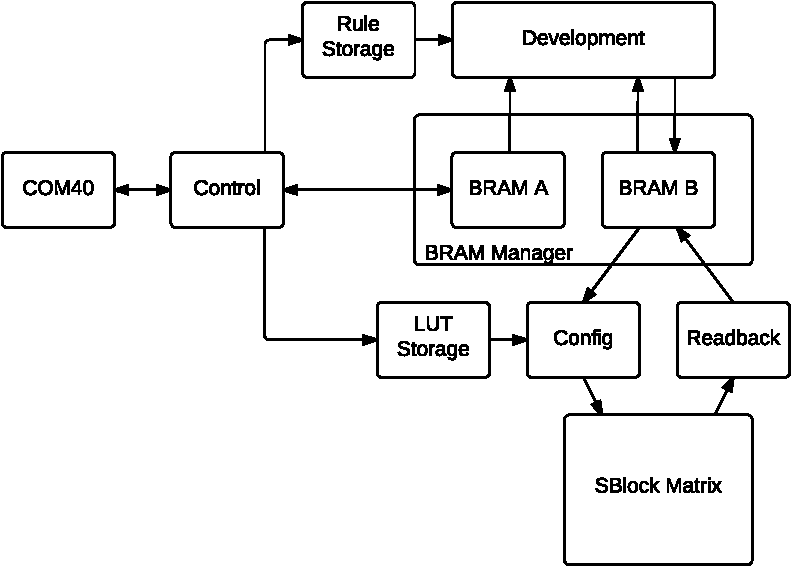
\includegraphics[width=0.48\textwidth]{figures/overview-djupdal}
    \caption{High-level block diagram of the hardware platform after Djupdal's original work.}
    \label{fig:overview-djupdal}
\end{figure}

\todo{detailed description}

\todo{clock domains}

\todo{also software}

\subsection{Extension}

There was one major bottleneck in the original design.
To calculate the fitness of an individual, the state of each cell had to be transfered to the computer over the PCI interface.
Having a dedicated hardware unit would greatly improve the performance.
Additionaly, it was desired to have more information about the development process.
The task of realizing this fell to Aamodt \cite{aamodt2005sblock}.

An overview of the hardware platform with Aamodt additions is shown in \figurename~\ref{fig:overview-aamodt}.
The additions consists of a run-step function that calculates the number of live cells, BRAM to store the numbers, a fitness function, and two information outputs from the development unit.

\begin{figure}[!ht]
    \centering
    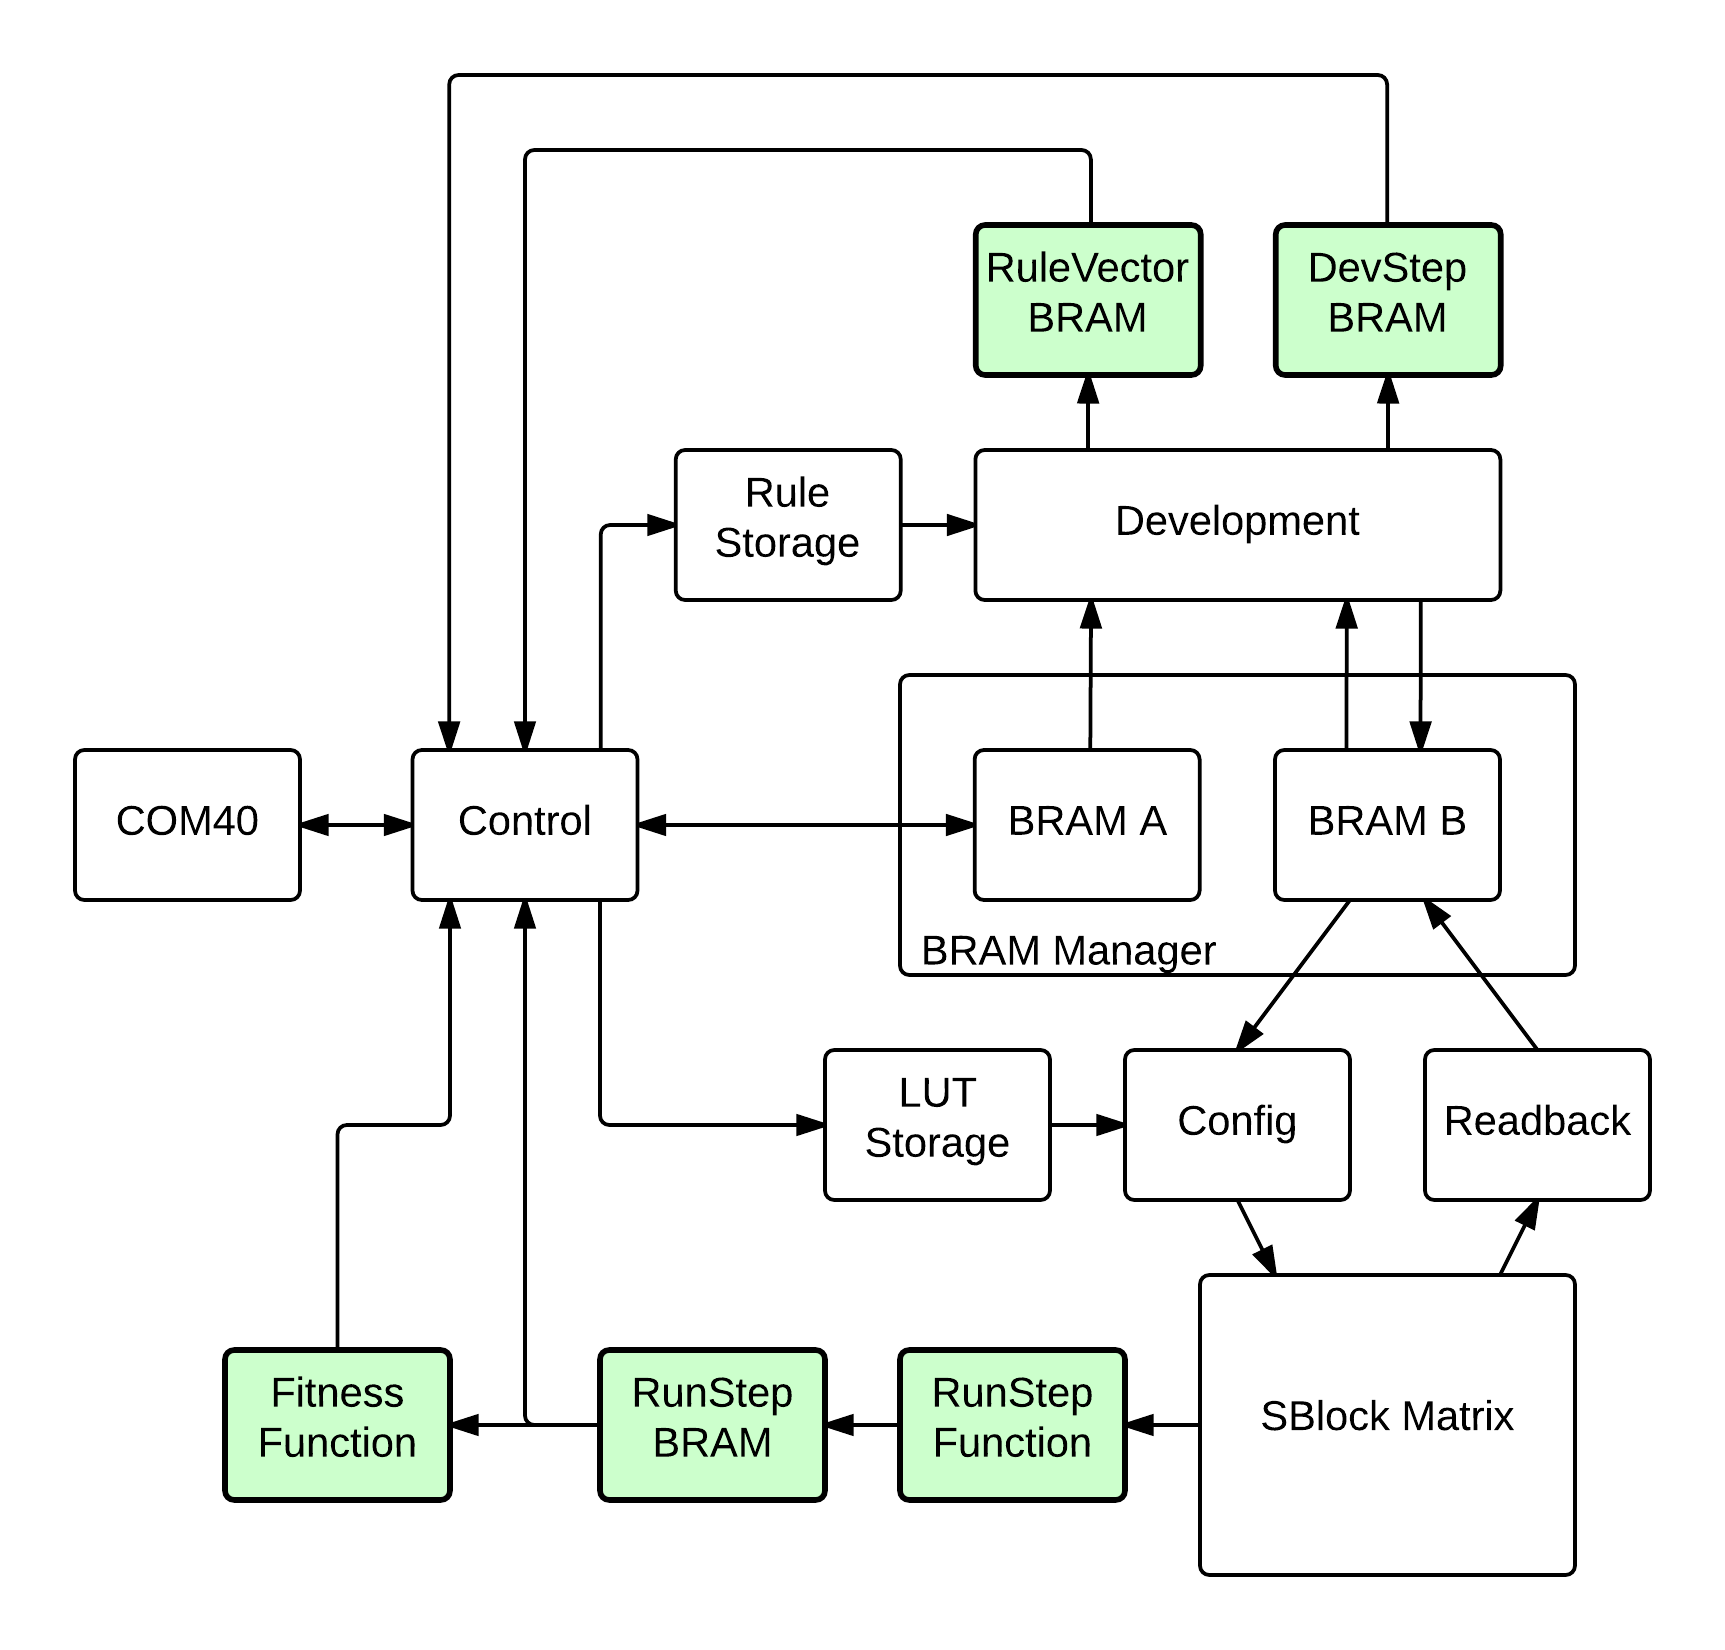
\includegraphics[width=0.48\textwidth]{figures/overview-aamodt}
    \caption{High-level block diagram of the hardware platform after Aamodt's work. Additions are highlighted in green.}
    \label{fig:overview-aamodt}
\end{figure}

\todo{detailed description}

\todo{also software}

\subsection{Renovation}

In expectation of receiving new hardware with a larger and faster FPGA, there was a demand to optimize the platform by take advantage of the increased resource pool.
Extending the platform into the third dimension was also a lucrative thought, as doing so allows more complex signal pathways to form within the cellular automata.
It was also desired to have a discrete fourier transform for interpretation of the RSF data; it should give very useful data according to Berg's research \cite{berg2013ca}.
The task of realizing this was taken on by Støvneng \cite{stovneng2014sblock}.

An overview of the hardware platform with Støvnengs additions and optimizations is shown in \figurename~\ref{fig:overview-stovneng}.
The only addition is the DFT, but nearly all units has been optimized, yielding a speedup of 4 for most operations.

\begin{figure}[!ht]
    \centering
    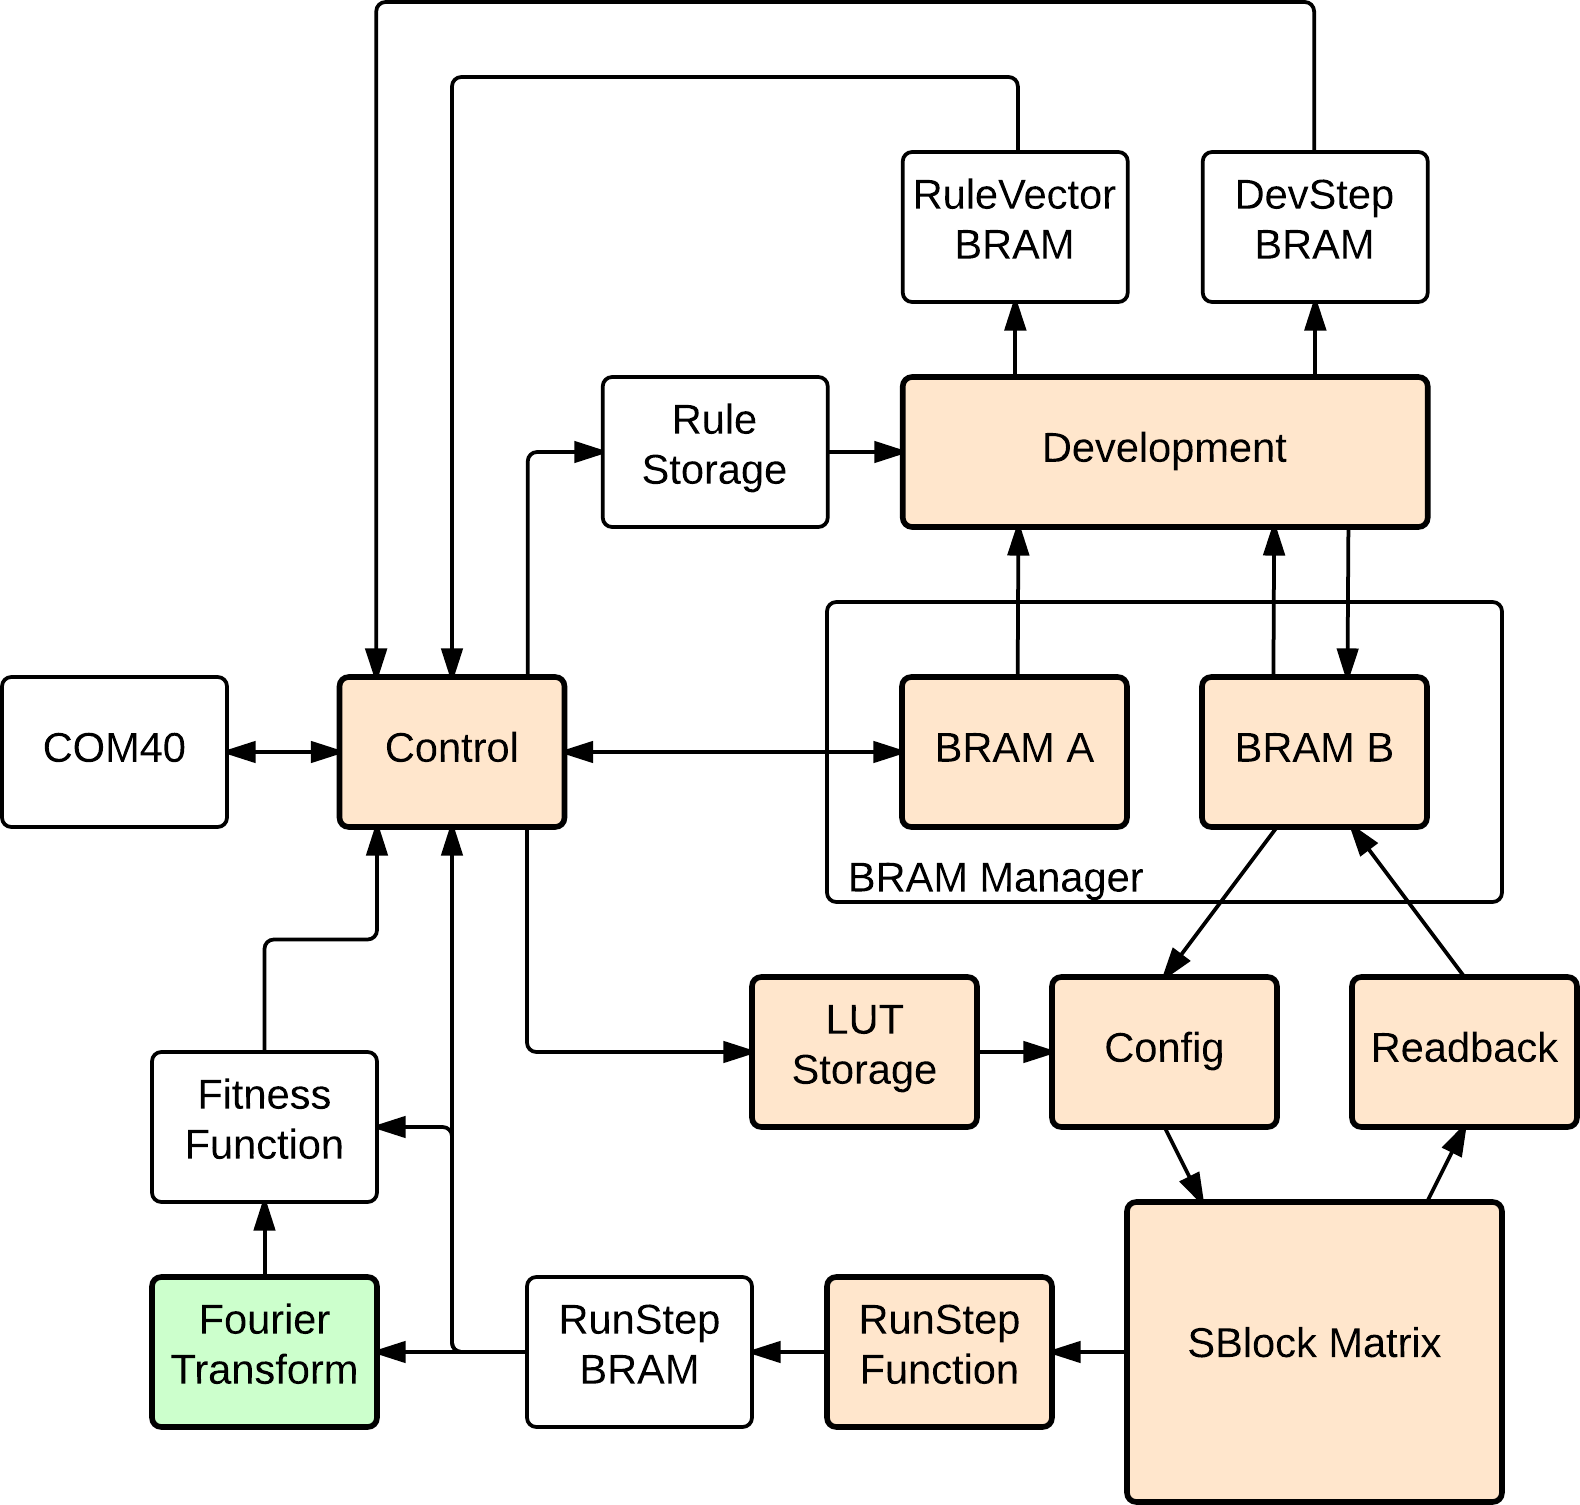
\includegraphics[width=0.48\textwidth]{figures/overview-stovneng}
    \caption{High-level block diagram of the hardware platform after Støvneng's work. Additions are highlighted in green, and optimizations and 3D modifications in orange.}
    \label{fig:overview-stovneng}
\end{figure}

\todo{detailed description}

\todo{also software}

Unfortunately, due to some challenges with manufacturing, Støvneng was unable to get hold of the new hardware for the duration of his project.
The system was therefore only verified in simulation, and the PCI communication unit was not upgraded for the PCI Express connection on the new board.

